\documentclass[12pt]{beamer}
%%%%%%%%%%%%%%%%%%%%%%%%%%%%%%%%%%%%%%%%%%%%%%%%%%%%%%%%%%%%%%%%%%%%%%%%%%%%%%%%%%%%%%%%%%%%%%%%%%%%%%%%%%%%%%%%%%%
% Appearance
\mode<presentation>
{
	\usetheme{CambridgeUS}
	\usecolortheme{whale}
	\setbeamercovered{transparent}
}
% Redefine beamer colors
% Captions and titles
\setbeamertemplate{caption}{\raggedright\insertcaption} 
\setbeamercolor{frametitle}{fg=cyan!90!black}
\setbeamercolor{title}{bg=cyan!90!black}

\setbeamercolor{palette primary}{fg=white, bg=cyan!70!black}
\setbeamercolor{palette secondary}{fg=white, bg=cyan!50!black}
\setbeamercolor{palette tertiary}{fg=white, bg=cyan!90!black}
% Outline slide
\setbeamertemplate{section in toc}[circle]
\setbeamerfont{section number projected}{family=\rmfamily,series=\bfseries,size=\normalsize}
\setbeamercolor{section number projected}{bg=cyan!90!black,fg=white}
% Itemize list
\setbeamertemplate{itemize item}[circle]
\setbeamertemplate{itemize subitem}[circle]
\setbeamercolor{itemize item}{fg=cyan!70!black}
\setbeamercolor{itemize subitemitem}{fg=cyan!90!black}
%%%%%%%%%%%%%%%%%%%%%%%%%%%%%%%%%%%%%%%%%%%%%%%%%%%%%%%%%%%%%%%%%%%%%%%%%%%%%%%%%%%%%%%%%%%%%%%%%%%%%%%%%%%%%%%%%%%
\usepackage[english]{babel}
% or whatever
\usepackage[latin1]{inputenc}
% or whatever
\usepackage{array} % To vertically center tabular content 
\usepackage{times}
%\usepackage[T1]{fontenc}

%%%%%%%%%%%%%%%%%%%%%%%%%%%%%%%%%%%%%%%%%%%%%%%%%%%%%%%%%%%%%%%%%%%%%%%%%%%%%%%%%%%%%%%%%%%%%%%%%%%%%%%%%%%%%%%%%%%%
%\usepackage{tikz}
\usepackage{pgfplots}
\pgfplotsset{every axis/.append style={line width=1pt}}
\usetikzlibrary{shapes,shadows,arrows,backgrounds,patterns,positioning,automata,calc,decorations.markings,decorations.pathreplacing,bayesnet,arrows.meta}
\usepackage{amsmath,amssymb,mathrsfs,amsfonts,amsthm} % for maths
\usepackage{graphicx}
\usepackage{eucal}    % for curly math letter symbols
\usepackage{amssymb}  % for ams symbols
\usepackage{pifont}
\usepackage{color} %Invoke options usenames,dvipsnames for larger color choice
\usepackage{microtype} % Slightly tweak font spacing for aesthetics
\usepackage{multicol} % Used for the two-column layout of the document
%%%%%%%%%%%%%%%%%%%%%%%%%%%%%%%%%%%%%%%%%%%%%%%%%%%%%%%%%%%%%%%%%%%%%%%%%%%%%%%%%%%%%%%%%%%%%%%%%%%%%%%%%%%%%%%%%%%%
\usepackage[backend=bibtex,style=ieee]{biblatex} % bibliography
\bibliography{Bibliography-thesis}
\renewcommand*{\bibfont}{\footnotesize}
%%%%%%%%%%%%%%%%%%%%%%%%%%%%%%%%%%%%%%%%%%%%%%%%%%%%%%%%%%%%%%%%%%%%%%%%%%%%%%%%%%%%%%%%%%%%%%%%%%%%%%%%%%%%%%%%%%%%
\title[Identification of immune cell migration] % (optional, use only with long paper titles)
{Modelling and Identification of Immune Cell Migration during the Inflammatory response}
\author[A. Kadochnikova]{A. Kadochnikova\inst{1}}
\institute[ACSE,TUoS]{\inst{1}
  Department of Automatic Control and Systems Engineering\\
  The University of Sheffield}
\date[21/06/2019]{21 June 2019}

\pgfdeclareimage[height=1cm]{university-logo}{UoSarms.pdf}
\logo{\pgfuseimage{university-logo}}


%\newcommand\id{\ensuremath{\mathbbm{1}}} 
%\DeclareMathOperator{\E}{\mathbb{E}}
%\DeclareMathOperator{\eye}{\mathbb{I}}
%\DeclareMathOperator{\zeros}{\mathbb{O}}
%\DeclareMathOperator{\tr}{\textrm{tr}}
%\DeclareMathOperator{\vvec}{\textrm{vec}}
%\DeclareSymbolFontAlphabet{\mathcal} {symbols}
%\DeclareSymbolFont{symbols}{OMS}{cm}{m}{n}

\begin{document}
\begin{frame}
  \titlepage
\end{frame}
\begin{frame}{Outline}
  \tableofcontents[hideallsubsections]
  % You might wish to add the option [pausesections]
\end{frame}

% - Exactly two or three sections (other than the summary).
% - At *most* three subsections per section.
% - Talk about 30s to 2min per frame. So there should be between about
%   15 and 30 frames, all told.

\section{Literature Review}
\subsection{Neutrophils in inflammatory response}

\subsection{Mathematical modelling of chemotaxis}

\subsection{Statistical inference methods}
\begin{frame}{Problems addressed in the thesis}
\begin{itemize}
	\item Formulate a finite-order model of heterogeneous cell dynamics that would incorporate the influence of unmeasurable chemoattractant concentration.
	\item Derive a statistical framework for estimating the hidden environment driving objects with hybrid dynamics.
	\item Simultaneously estimate the shape of chemoattractant concentration field and cell modes.
	\item Utilize the framework for processing \textit{in vivo} tracking data obtained for different types of wounds and stages of inflammation.
\end{itemize}
\end{frame}

\begin{frame}{Problems addressed in the thesis}
\begin{itemize}
	\item Formulate a state space model of cell morphodynamics to interpret AKT tracking data
	\item Estimate model parameters within maximum likelihood framework based \textit{in vivo} tracking data..
	\item Extend the model to include the dynamics of AKT concentration along the boundary.
\end{itemize}
\end{frame}

\begin{frame}{Limitations}

  \begin{itemize}
  	\item Minimise prior assumptions about the environment.
  	\item Minimise prior assumptions intacellular regulators.
  	\item Ensure identifiability of models by keeping the number of unknown parameters low. 
  	\end{itemize}
\end{frame}
\subsection{Identified gaps in literature}

\section{Chemoatractant field inference}

\subsection{Modelling cell-environment interaction}

\begin{frame}
	\begin{itemize}
	\uncover<2->{\item Randomness of motion impedes precise assessment of stimuli gradient by an individual, yet average behaviour of cells in population reflects it with remarkable accuracy.}
	\uncover<3->{\item Model for concentrations:
\begin{equation*}\label{KS1}
\frac{\delta b}{dt} = \nabla(\mu(s)\nabla(b)) - \nabla(\chi(s)b\nabla s);
\end{equation*}
\begin{equation*}\label{KS2}
\frac{\delta s}{dt} = D\nabla^2 s - f(b,s), 
\end{equation*}	
$b=b(x,t)$ - concentration of cells; \\
$s=s(x,t)$ - concentration of attractant;\\
$\mu$ - cell diffusion coefficient, $\chi$ - attractant coefficient.}
\end{itemize}
\end{frame}

\begin{frame}{State-space representation}
Individual cell dynamics \cite{Kadirkamanathan2012}:
\begin{equation*}\label{eq_dyn}
\mathbf{x}_{t+1} = A\mathbf{x}_t + B\mathbf{u}_t + G\omega_t
\end{equation*}
\begin{equation*}\label{eq_meas}
\mathbf{y}_t = C\mathbf{x}_t + \upsilon_t,
\end{equation*}
where
\begin{equation*}
\mathbf{u}= \nabla \mathbf{U}.
\end{equation*}
The hidden environment is parametrised with $n_b$ cardinal cubic B-splines $\beta_h(s)$ with an assigned scaling parameter $\theta_h$.
\end{frame}

%\begin{frame}{Cell modes}
%Neutrophil behaviour during recruitment stage can be described by a set of models.
%\begin{columns}
%	\begin{column}{0.5\textwidth}
%		Types of random walk \cite{Jones2015}:
%		\begin{itemize}
%			\item biased, persistent
%			\item biased, non-persistent
%			\item non-biased, persistent
%			\item non-biased, non-persistent
%		\end{itemize}
%	\end{column}
%	\begin{column}{0.5\textwidth}
%		Based on the interaction \\with the environment:
%		\begin{itemize}
%			\item driven by the field
%			\begin{itemize}
%				\item KS model
%				\item Potential Field model
%			\end{itemize}
%			\item insensitive - RW
%			\item stationary - RW
%		\end{itemize}
%		
%	\end{column}
%\end{columns}
%\end{frame}

%\begin{frame}{Defining assumptions}
%\begin{itemize}
%	\item Cell velocity is proportional to the gradient of the field (K-S model).
%	\item Cell acceleration is proportional to the gradient of the field (potential field model - analogous to path planning in robotics).
%	\item The hidden environment is time-invariant.
%	\item Each cell at each time can be in one of three modes: responsive, not responsive, stationary.
%\end{itemize}
%\end{frame}


%\begin{frame}{Jump Markov Linear system}
%%\begin{equation*}\label{eq_dyn1}
%%\mathbf{x}_{t+1} = A(M^j)\mathbf{x}_t + B(M^j)\mathbf{u}_t + G(M^j)\mathbf{w}_t, \quad \mathbf{w}_t \sim \mathcal{N}(0,\sigma(M^j)).
%%\end{equation*}
%%Cell modes:
%%\begin{equation*}
%%M^1: A = \begin{bmatrix}
%%\eye & T \eye \\ \zeros & \eye
%%\end{bmatrix}; B = \begin{bmatrix}
%%\frac{T^2}{2} \eye \\ \zeros
%%\end{bmatrix} \textrm{- responding to the environment}
%%\end{equation*} 
%%\begin{equation*}
%%M^2: A = \begin{bmatrix}
%%\eye & T \eye \\ \zeros & \zeros
%%\end{bmatrix}; B = \begin{bmatrix}
%%\zeros \\ \zeros
%%\end{bmatrix} \textrm{- not responsive, diffusing}
%%\end{equation*}
%%\begin{equation*}
%%M^3: A = \begin{bmatrix}
%%\eye & T \eye \\ \zeros & \zeros
%%\end{bmatrix}; B = \begin{bmatrix}
%%\zeros \\ \zeros
%%\end{bmatrix} \textrm{- stationary}
%%\end{equation*}
%%\begin{equation*}
%%\sigma(M^3) \ll \sigma(M^1) < \sigma(M^2)
%%\end{equation*}
%\end{frame}

%\begin{frame}{Jump Markov Linear System}
%\begin{columns}
%\begin{column}{0.6\textwidth}
%\scalebox{0.8}{\input{Tikzes/Markov_chain_switch.tikz}}
%\end{column}
%\begin{column}{0.4\textwidth}
%\begin{itemize}
%	\item \textit{k} - cell index
%	\item t - time 
%	\item $\pi_j$ - probability of $M^j$ at time $t = 0$
%	\item $\phi_{ij}$ - probability of transitioning from $M^i$ to $M^j$
%	\item $\psi_j$ - probability of state $x^{k}_{t}$	
%\end{itemize}
%\end{column}
%\end{columns}
%\end{frame}
%
%\section{Estimation of chemoattractant concentration}
%\subsection{Data}
%\begin{frame}
%Available tracking data from zebrafish inflammation model:
%\begin{itemize}
%	\item Mild injury (6 datasets)
%	\item Severe injury (3 datasets)
%	\item Tail fin nick (4 datasets)
%	\item Reverse migration (6 datasets)
%\end{itemize}
%\end{frame}

%\subsection{Estimation Framework}
%
%\begin{frame}
%\begin{figure}
%\centering
%\begin{tikzpicture}[->, >=stealth', auto, semithick, node distance=5em]
%\tikzstyle{block} = [rectangle, draw, fill=white, 
%text width=7em, text centered, rounded corners, minimum height=2em]
%\tikzstyle{line} = [draw, -latex']	
%\node[block,align=center] at (1.5,7) (A1){\small Neutrophil tracking \\ data};
%\node[block,align=center] at (1.5,4.8) (A2){\small Parametrised model \\ of the field};
%\node[block,align=center] at (1.5,2.3) (A3){\small Set of SSMs describing\\ cell dynamics \\ $\{M^1, M^2, M^3\}$};
%\node[align=center] at (5.75,6) (A4){\small Inference framework};
%\node[block,align=center] at (5.75,5) (A5){\small Cell state \\estimation};
%\node[block,align=center] at (5.75,3.5) (A6){\small Field \\inference};
%\node[block,align=center] at (10,5.45) (A7){\small Inferred shape of the\\chemoattractant field};
%\node[block,align=center] at (10,3.2) (A8){\small Decision about\\ the cell mode\\ at each time};
%\draw[red] (3.75,6.5) rectangle (7.75,2.7);
%\node at (5.75,6.35) (A9){};
%\node at (5.75,2.85) (A10){};
%\node at (3.9,4.8) (A11){};
%\node at (7.6,5.45) (A12){};
%\node at (7.6,3.2) (A13){};
%%% arrows
%\draw (A1) -| (A9); 
%\draw (A2) -- (A11); 
%\draw (A3) -| (A10); 
%\draw (A12) -- (A7); 
%\draw (A13) -- (A8); 
%\path
%(A5.east) edge[dashed,bend left=30] (A6.east);
%\path
%(A6.west) edge[dashed,bend left=30] (A5.west);
%\end{tikzpicture}
%\end{figure}	
%\end{frame}

%\subsection{Results}
%\begin{frame}
%\begin{columns}
%	\begin{column}{0.5\textwidth}
%		\centering
%		\scalebox{0.25}{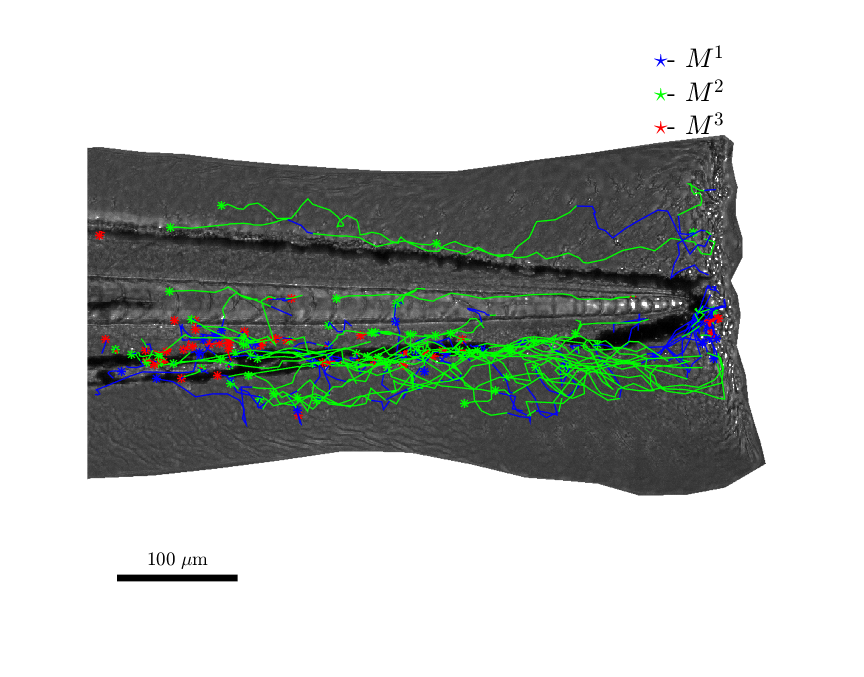
\includegraphics{Figures/modes_f3_mild.png}}\\
%		\scalebox{0.25}{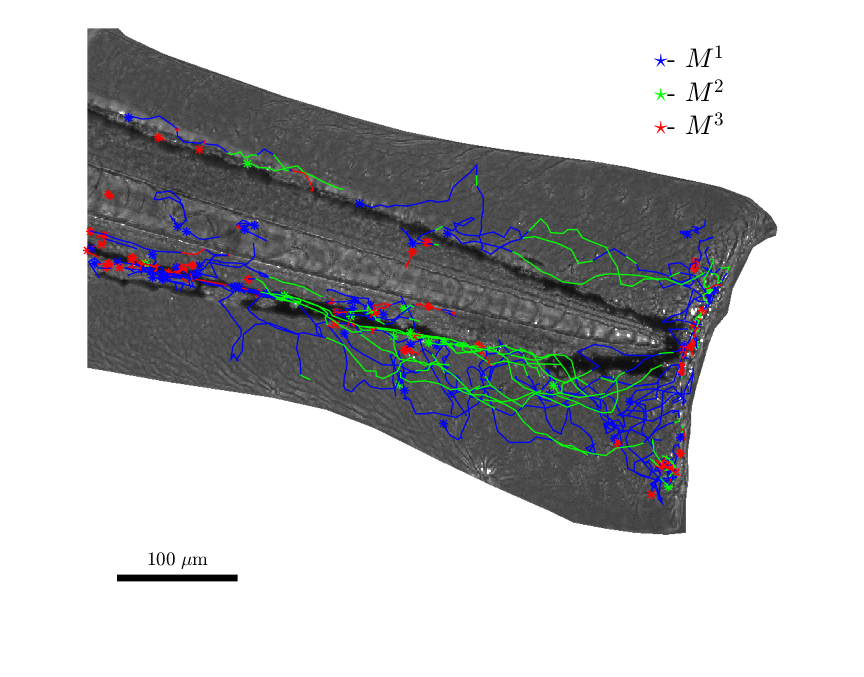
\includegraphics{Figures/tracks_fish_5.png}}
%	\end{column}
%	\begin{column}{0.5\textwidth}
%		\centering
%		\scalebox{0.25}{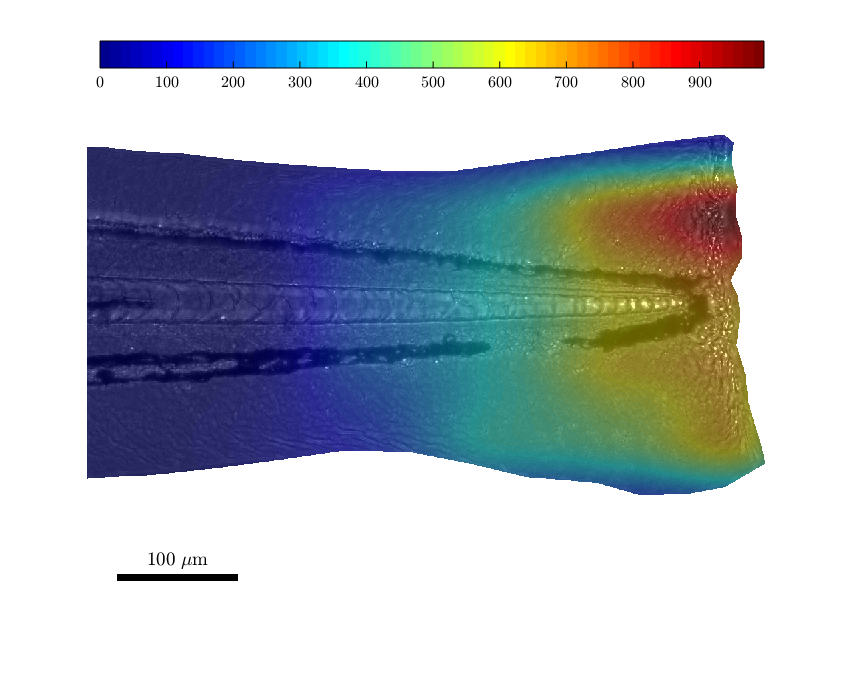
\includegraphics{Figures/field_fish_3.png}}	\\
%		\scalebox{0.25}{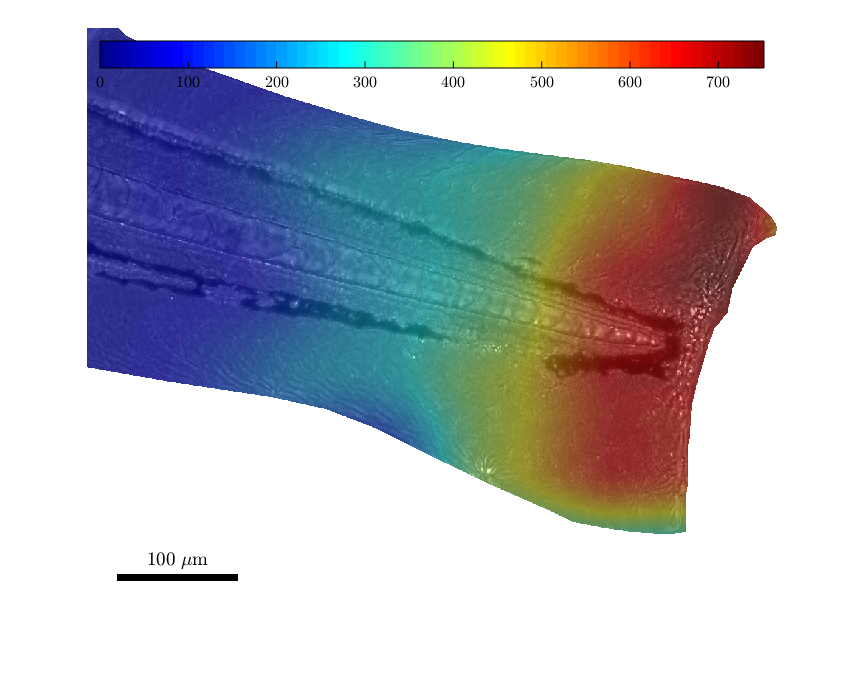
\includegraphics{Figures/field_fish_5.png}}	
%	\end{column}
%\end{columns}
%\end{frame}
%
%\begin{frame}
%\begin{columns}
%	\begin{column}{0.5\textwidth}
%		\centering
%		\scalebox{0.2}{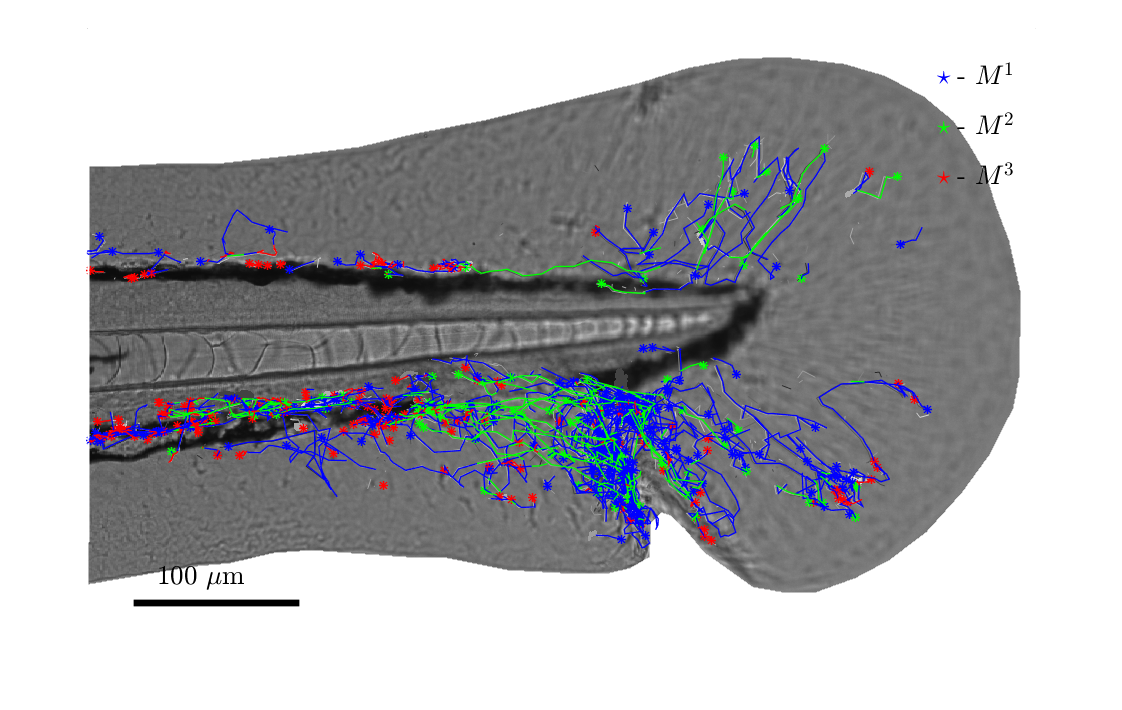
\includegraphics{Figures/h6_tracks.png}} \\
%		\scalebox{0.2}{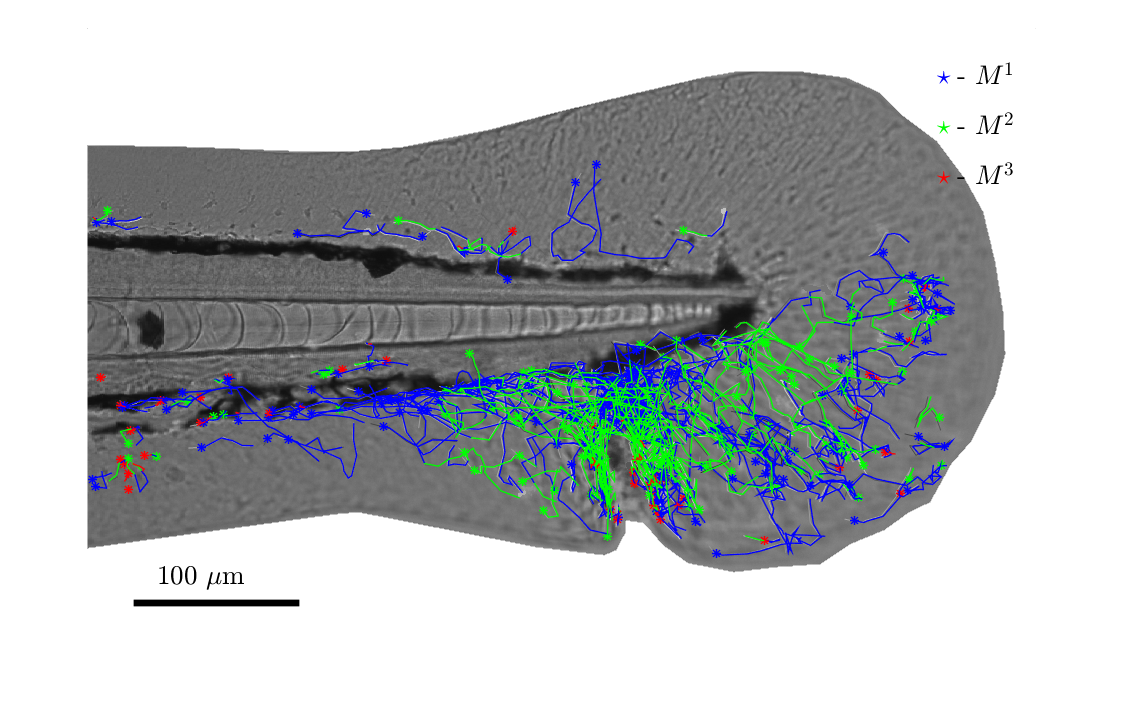
\includegraphics{Figures/h4_tracks.png}}
%	\end{column}
%	\begin{column}{0.5\textwidth}
%		\centering
%		\scalebox{0.2}{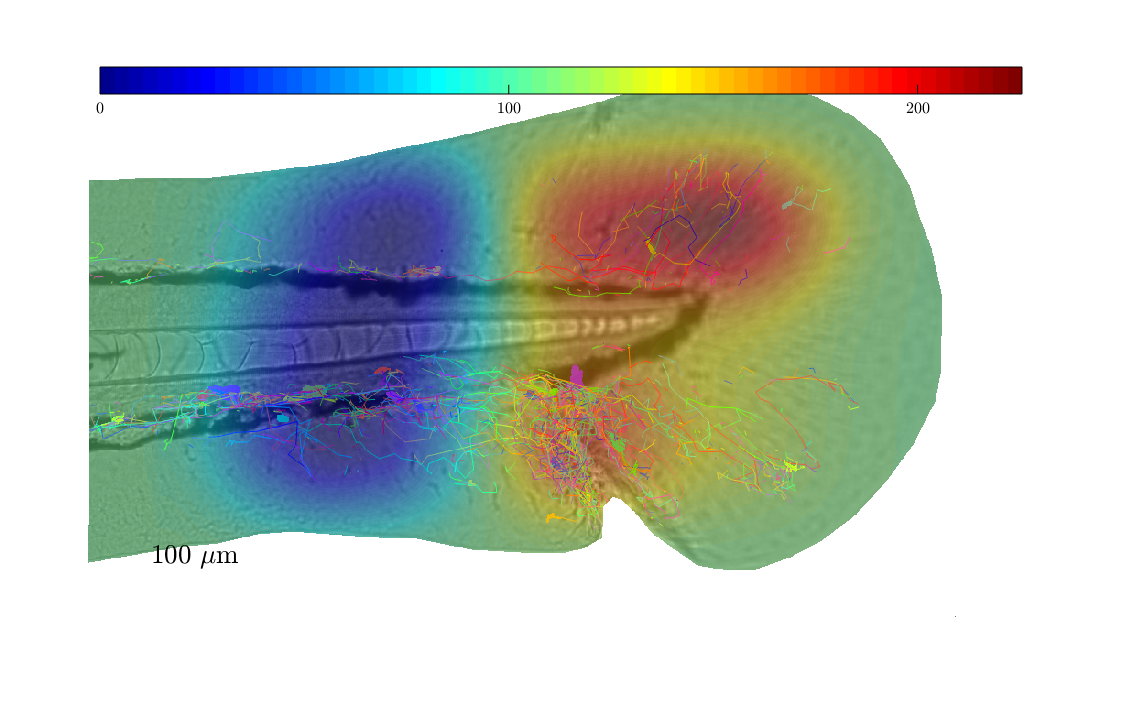
\includegraphics{Figures/h6_field.png}} \\
%		\scalebox{0.2}{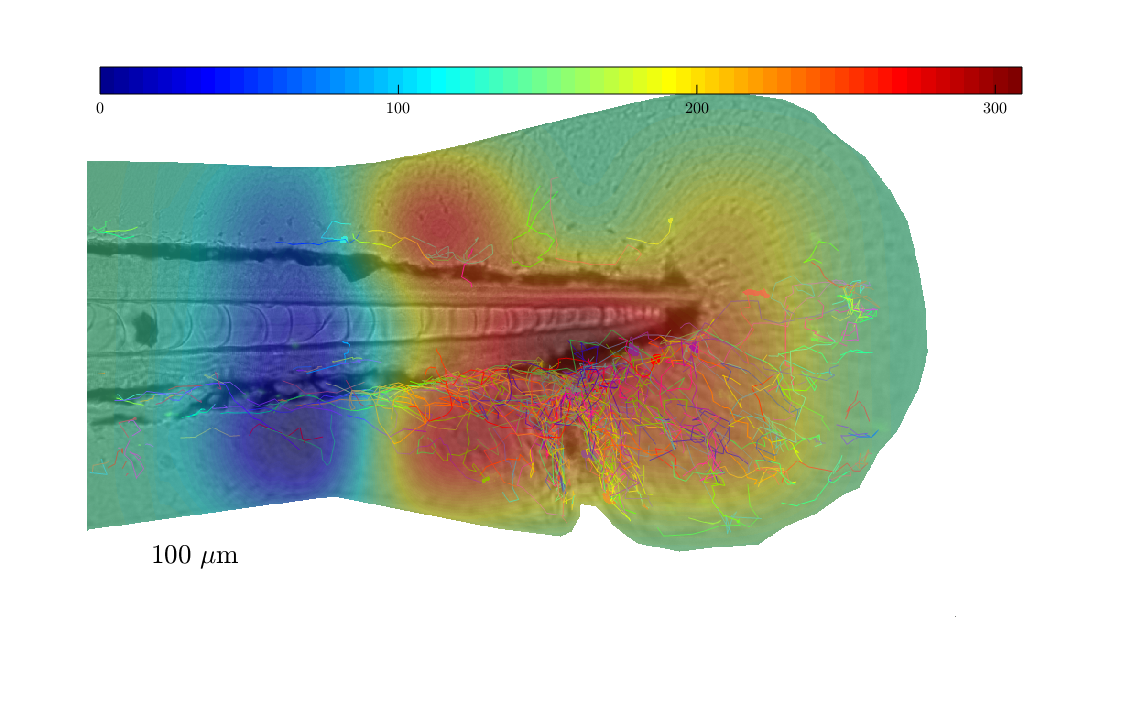
\includegraphics{Figures/h4_field.png}}	
%	\end{column}
%\end{columns}
%\end{frame}
%
%\begin{frame}
%Model of fugetaxis: $ \mathbf{u}_t = - \nabla \mathbf{U}$
%\begin{columns}
%	\begin{column}{0.5\textwidth}
%		\centering
%		\scalebox{0.2}{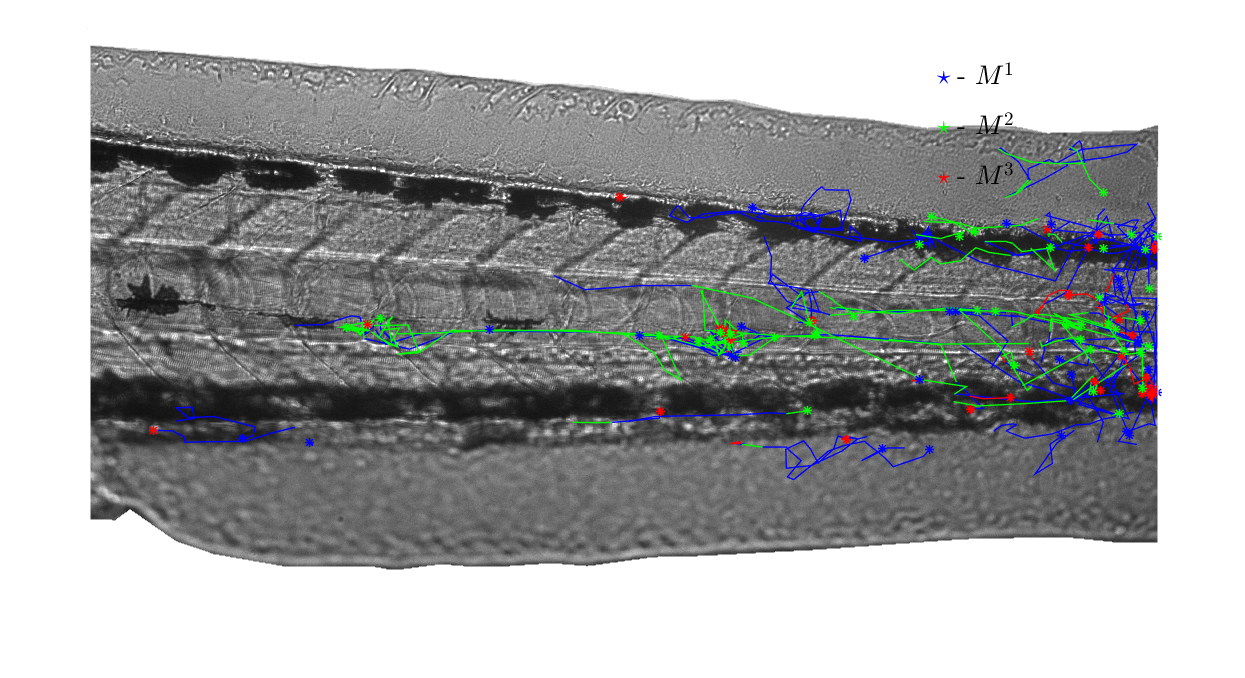
\includegraphics{Figures/trcks_f2.png}} \\
%	\end{column}
%	\begin{column}{0.5\textwidth}
%		\centering
%		\scalebox{0.2}{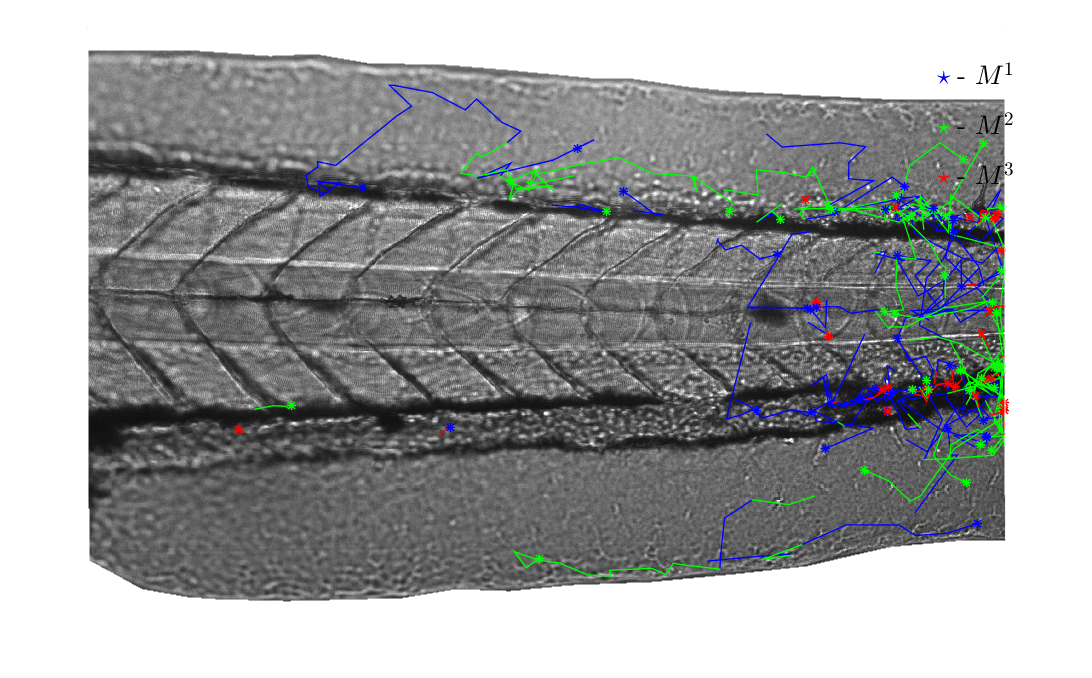
\includegraphics{Figures/trcks_f3.png}} \\	
%	\end{column}
%\end{columns}
%Conflicting environments on inflammation resolution stage?
%\end{frame}

\section{Identification of cell morphodynamics}
\subsection{Motivation}
\begin{frame}
\begin{columns}
	\begin{column}{0.4\textwidth}
		\centering
		\scalebox{0.2}{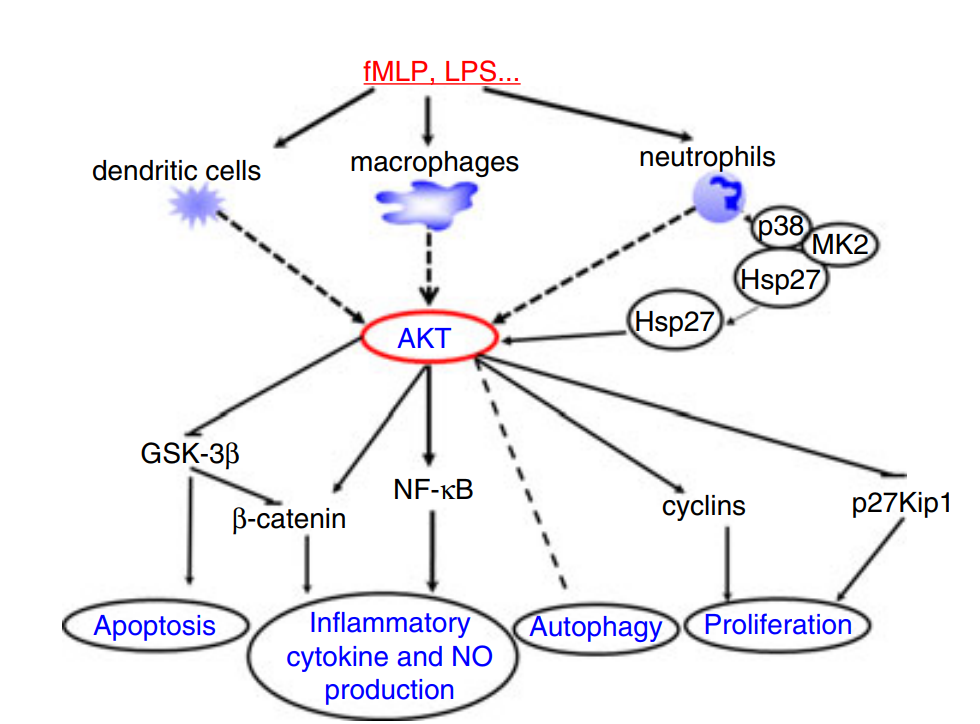
\includegraphics{Figures/aktrole.png}}
	\end{column}
	\begin{column}{0.6\textwidth}
\begin{itemize}
	\item PI3K/AKT signalling pathway plays critical role in neutrophil migration driven by intermediary chemoattractants \cite{Zhang2013}.
	\item AKT2 KO neutrophils exhibit reduced chemotactic activity \cite{Chen2010}.
	\item Enchanced PI3K/AKT activation induced by p38 MAPK inhibitors is causally related to the increase in neutrophil chemotaxis \cite{Heit2002}.
\end{itemize}	
	\end{column}
\end{columns}
\end{frame}

\subsection{Data}
\begin{frame}
\centering
\begin{columns}
	\begin{column}{0.5\textwidth}
		\centering
		\scalebox{0.4}{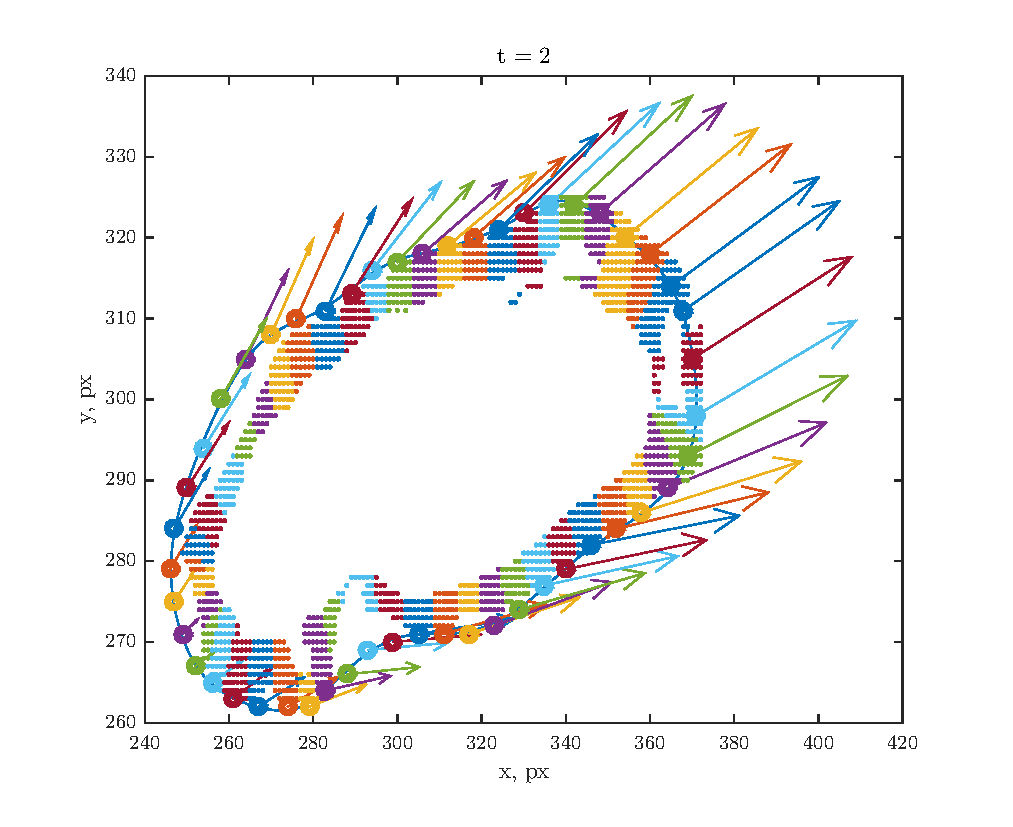
\includegraphics{Figures/akt_try1_c2_t2_Intens_speed.eps}}		
	\end{column}
	\begin{column}{0.5\textwidth}
	\scalebox{0.4}{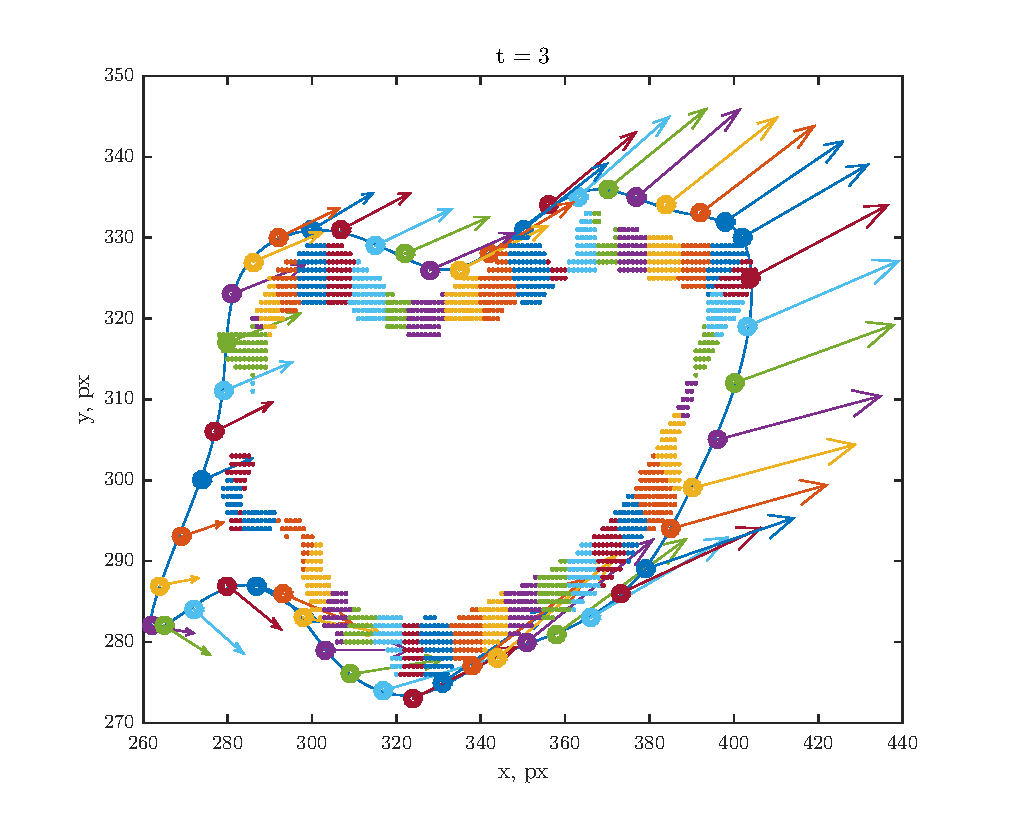
\includegraphics{Figures/akt_try1_c2_t3_Intens_speed.eps}}	
	\end{column}
\end{columns}
\end{frame}

\subsection{Mathematical model}
\begin{frame}{Cell boundary evolution}
\begin{equation*}
\mathcal{F} = (\mathcal{F}_{\textrm{visc}} + \mathcal{F}_{\textrm{pro}} + \mathcal{F}_{\textrm{ten}} + \mathcal{F}_{\textrm{vol}})\nu,
\end{equation*}
\begin{itemize}
	\item \textbf{\textit{Protrusive force}}. $\mathcal{F}_{\textrm{pro}}$ is proportional to the concentration of chemical species active along the cell boundary \cite{Shao2010}. 
	\item \textbf{\textit{Surface tension}}. $\mathcal{F}_{\textrm{ten}}$ corresponds to surface energy that prevents cell membrane from stretching. \cite{Elliott2012}.
	\item \textbf{\textit{Volume conservation}}. $\mathcal{F}_{\textrm{vol}}$ balances small volume changes caused by boundary evolution. Computed as a hard constant \cite{Elliott2012}, or dependant on changes of the cell area \cite{Iglesias2013}.
	\item \textbf{\textit{Viscous force}}. $\mathcal{F}_{\textrm{visc}}$ opposes cell motion, proportional to current velocity.
\end{itemize}
$\quad$\\
$\quad$
\end{frame}

\begin{frame}{Signalling Network}
\begin{columns}
\begin{column}{0.6\textwidth}
	\begin{figure}
		\scalebox{0.25}{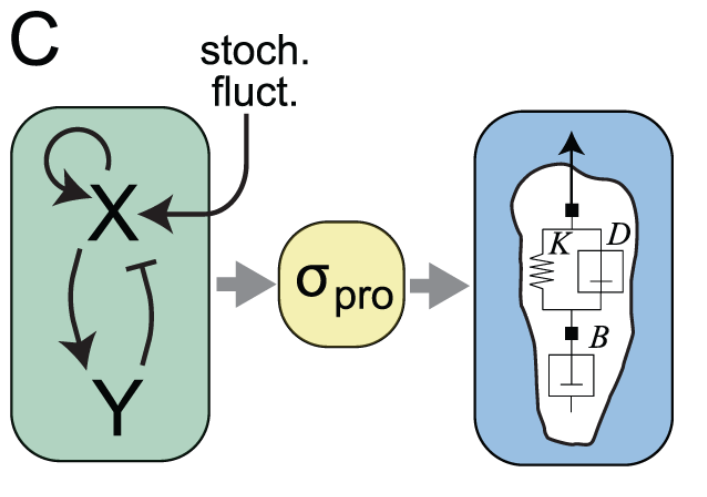
\includegraphics{Figures/en.png}}
		\caption{\small Excitation network diagram in \cite{Iglesias2013}.} 
	\end{figure}
\end{column}
\begin{column}{0.4\textwidth}
	\begin{figure}
		\scalebox{0.2}{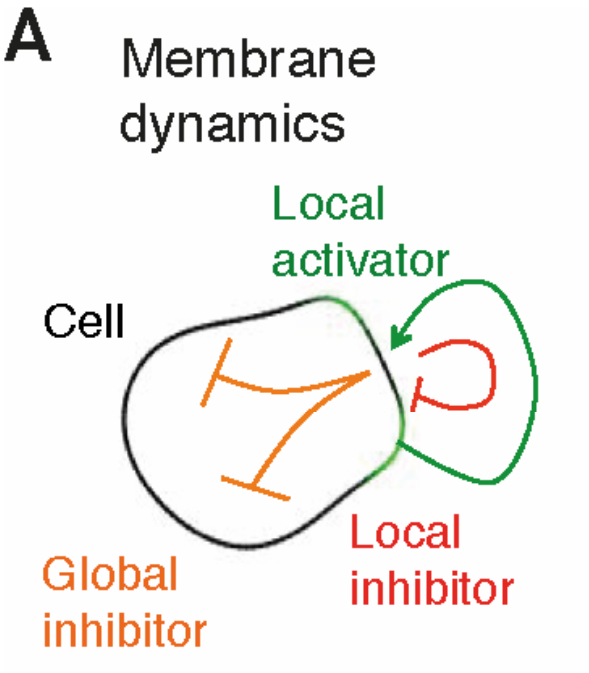
\includegraphics{Figures/membrane_dyn.png}}
		\caption{Membrane dynamics diagram in \cite{Endres2017}.} 
	\end{figure}
\end{column}
\end{columns}
	$X$ - activator responding to amplified signal from cell surface \\$Y$ - provides negative feedback to $X$.\\ $\sigma_{\textrm{pro}}$ - protrusive force acting on cell boundary.
\end{frame}

\begin{frame}{Defining assumptions}
\begin{itemize}
	\item Fluorescence intensity of the cell image is representative of AKT concentration along the cell boundary.
	\item AKT is the only activator driving boundary evolution.
	\item Nodes on the cell boundary are equidistant. 
	\item Sensing of the local chemoattractant field is a stochastic process with reversion to mean.
\end{itemize}
\end{frame}

\begin{frame}{State space representation}
\begin{equation*}
\mathbf{v}_{t+1}^{k} = A\mathbf{v}_{t}^{k} + B\mathbf{u}_{t}^{k}+ \omega_{t}^{k}, \quad \omega_{t}^{k} \sim \mathcal{N}(0,Q)
\end{equation*}
\begin{equation*}
\mathbf{y}_{t}^{k} = C \mathbf{v}_{t}^{k} + \upsilon_{t}^{k},\quad \upsilon_{t}^{k} \sim \mathcal{N}(0,R).
\end{equation*}
\begin{itemize}
	\item $A = \alpha_{\textrm{vv}}, \quad$ $\quad B = \left[\alpha_{\textrm{pro}}, \alpha_{\textrm{ten}}, \alpha_{\textrm{vol}}\right]$.
	\item $u_{t}^{k} = \left[ e_{t}^{k}, \mathcal{K}_t, \Delta\mathcal{A}_t \right]^\top$, where
	\begin{itemize}
		\item $e_{t}^{k}$ - local excitation;
		\item $\mathcal{K}_t$ - mean curvature;
		\item $\Delta\mathcal{A}_t = \mathcal{A}_t - \mathcal{A}_0$ - change in cell shape. 
	\end{itemize}
	\item $\lambda = \lbrace A, B, Q, R, \mathbf{v}_0, P_0 ) \rbrace$ - unknown parameters.
\end{itemize}
\end{frame}


\begin{frame}
\begin{columns}
	\begin{column}{0.5\textwidth}
		\begin{figure}
			\scalebox{0.8}{\input{Tikzes/vertnormals.tikz}}
			\caption{\small Cell normals.} 
		\end{figure}
	\end{column}
	\begin{column}{0.5\textwidth}
		\begin{figure}
			\scalebox{0.8}{\input{Tikzes/area1.tikz}}
			\caption{Cell area computation.} 
		\end{figure}
	\end{column}
\end{columns}
\end{frame}

\begin{frame}
\begin{columns}
	\begin{column}{0.5\textwidth}
		\begin{figure}
			\scalebox{0.8}{\input{Tikzes/normvelt3.tikz}}
			\caption{\small Normal velocity at t=3.} 
		\end{figure}
	\end{column}
	\begin{column}{0.5\textwidth}
		\begin{figure}
			\scalebox{0.8}{\input{Tikzes/normvelt4.tikz}}
			\caption{Normal velocity at t=4.} 
		\end{figure}
	\end{column}
\end{columns}
\end{frame}


\begin{frame}
\begin{columns}
	\begin{column}{0.5\textwidth}
		\begin{figure}
			\scalebox{0.7}{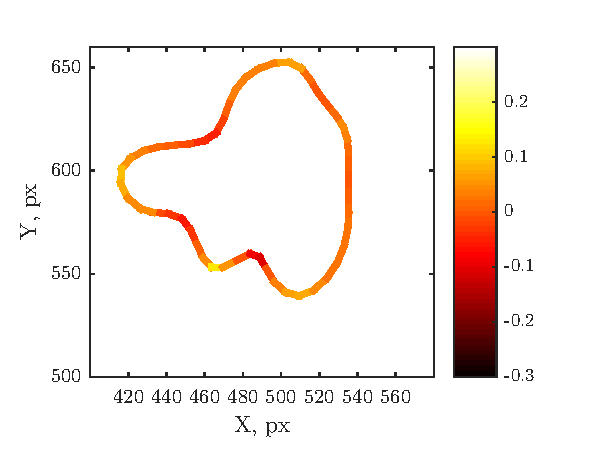
\includegraphics{Figures/curv3.eps}}
			\caption{\small Local curvature at t=3.} 
		\end{figure}
	\end{column}
	\begin{column}{0.5\textwidth}
		\begin{figure}
			\scalebox{0.7}{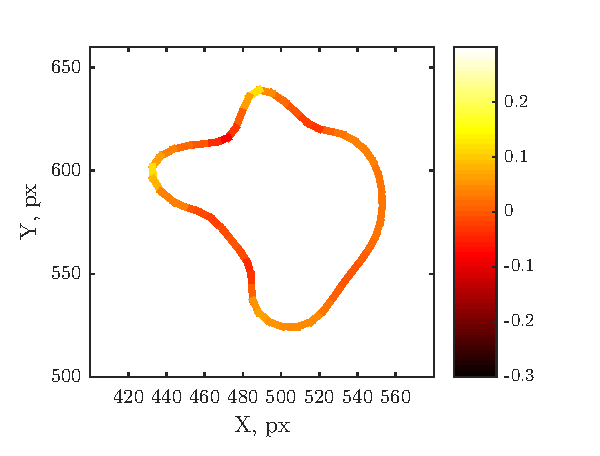
\includegraphics{Figures/curv4.eps}}
			\caption{Local curvature at t=4.} 
		\end{figure}
	\end{column}
\end{columns}
\end{frame}



%\subsection{Estimation algorithm}
%\begin{frame}
%\begin{itemize}
%	\item Initialise $\lambda^0$
%	\item Repeat until parameter convergence:
%	\begin{itemize}
%		\item Estimate states $\left[ \mathbf{v}, \mathbf{e} \right]$ (velocity, activator concentration)
%		\item Estimate parameters $\left[\lambda^i\right]$
%	\end{itemize} 
%\end{itemize}
%\end{frame}

\section{Conclusion}
\subsection{Contributions}
\begin{frame}
% Keep the summary *very short*.
\begin{itemize}
	\item
	Investigation of cell-environment interaction on different stages of inflammation on different spatial scales.
	\item
	A statistical framework for inference of the hidden environment driving objects with hybrid dynamics.
	\item
	Analysis of cell boundary evolution driven by intracellular signalling.
\end{itemize}
\end{frame}
\subsection{Future work}
\begin{frame}
\begin{itemize}
	\item Improve field estimation framework
	\item Consider time-variable field
\end{itemize}
\end{frame}
\begin{frame}{Disseminated results}
\begin{itemize}
\item
The EM estimation framework - a journal paper under peer review in \textit{IEEE Transactions on Signal Processing}.
\item
Chemoattractant field estimation (with linear model of cell dynamics) - a conference paper in \textit{IFAC IEEE CSS Symposium on System Identification, 2018}
\item
Chemoattractant field estimation (with switching model of cell dynamics) - a journal paper in preparation. Potential journals: \textit{PLoS One, Interface Focus, Bioinformatics}
\item Identification of cell morphodynamics - a conference paper (too empirical?)
\end{itemize}
\end{frame}

% All of the following is optional and typically not needed. 
\appendix
\section<presentation>*{\appendixname}
\subsection<presentation>*{References}

\begin{frame}[allowframebreaks]
\printbibliography
\end{frame}
\end{document}


